\documentclass{beamer}
\usepackage{beamerthemesplit}
\usetheme{SPbGU}
%{CambridgeUS}
% Выпишем часть возможных стилей, некоторые из них могут содержать
% дополнительные опции
% Darmstadt, Ilmenau, CambridgeUS, default, Bergen, Madrid, AnnArbor,Pittsburg, Rochester,
% Antiles, Montpellier, Berkley, Berlin
\usepackage{pdfpages}
\usepackage{amsmath}
\usepackage{cmap} % for serchable pdf's
\usepackage[T2A]{fontenc} 
\usepackage[utf8]{inputenc}
\usepackage[english,russian]{babel}
\usepackage{indentfirst}
\usepackage{amsmath}
\usepackage{dot2texi}
\usepackage{tikz}
\usepackage{graphicx}
\usetikzlibrary{shapes,arrows}
% Если у вас есть логотип вашей кафедры, факультета или университета, то
% его можно включить в презентацию.

%\usefoottemplate{\vbox{}}%  \tinycolouredline{structure!25}% {\color{white}\textbf{\insertshortauthor\hfill% \insertshortinstitute}}% \tinycolouredline{structure}% {\color{white}\textbf{\insertshorttitle}\hfill}% }}

%\logo{
\includegraphics[width=1cm]{SPbGU_Logo.png}}

%[GLR-анализатор]
\title[YaccConstructor]{Разработка средств реинжиниринга}
\subtitle[студроект]{Студенческий проект}
\institute[СПбГУ]{
Санкт-Петербургский государственный университет \\
Математико-Механический факультет \\
Кафедра системного программирования }

\lead[Григорьев Семён]{Григорьев Семён Вячеславович}
\date{2 мая 2012г.}

\begin{document}
{
    \begin{frame}
        \begin{center}
            {
\includegraphics[width=1cm]{SPbGU_Logo.png}}
        \end{center}
        \titlepage
    \end{frame}
}

\begin{frame}
	\transwipe[direction=90]
	\frametitle{О проекте}
	\begin{itemize}
		\item Название: YaccConctructor
		\item Сайт проекта: \href{http://recursive-ascent.googlecode.com} {http://recursive-ascent.googlecode.com}
		\item YaccConstructor -- это модульный инструмент для разработки парсеров и трансляторов для платформы .NET. Реализован на F\#. Основная область применения -- реинжиниринг программного обеспечения.
	\end{itemize}
\end{frame}

\begin{frame}
	\transwipe[direction=90]
	\frametitle{YaccConstructor}
	\begin{center}
        {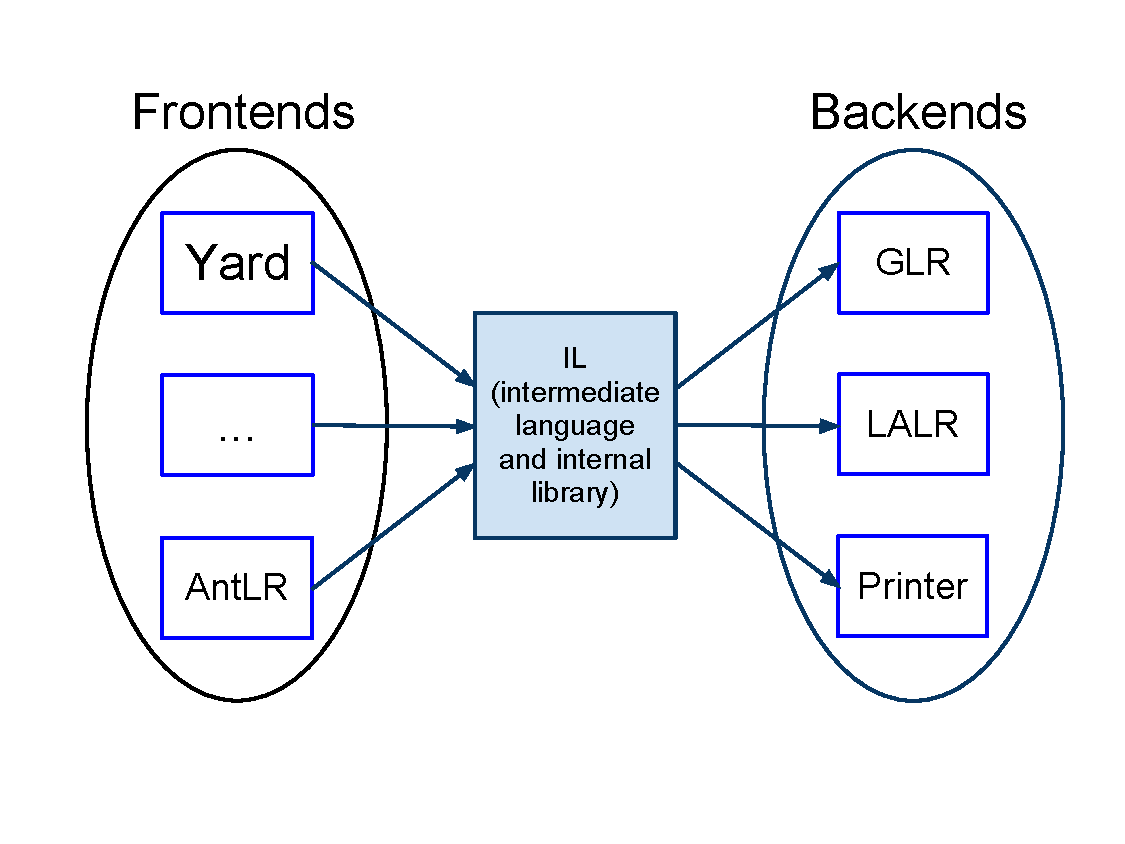
\includegraphics[width= 0.9\textwidth, height=\textheight]{diagrams/YC_general.pdf}}
    \end{center}
\end{frame}    

\begin{frame}
	\transwipe[direction=90]
	\frametitle{Участники}
	Участники студенческого проекта 2011-2012:
	\begin{itemize}
        \item Дейкин Александр
        \item Шенбин Илья
    \end{itemize}
\end{frame}    

\author[Дейкин Александр]{}

\begin{frame}
	\transwipe[direction=90]
	\frametitle{Задача}
	Доработка модульной архитектуры
	\begin{itemize}
        \item Анализ модулей и выделение общей функциональности
        \item Реализация общего предка и вынесение общей функциональности
    \end{itemize}
\end{frame}    

\begin{frame}
	\transwipe[direction=90]
	\frametitle{Модули  YaccConstructor}
	Модули, управляющие загрузкой компонент. Изначальный вариант.
	\begin{center}
        {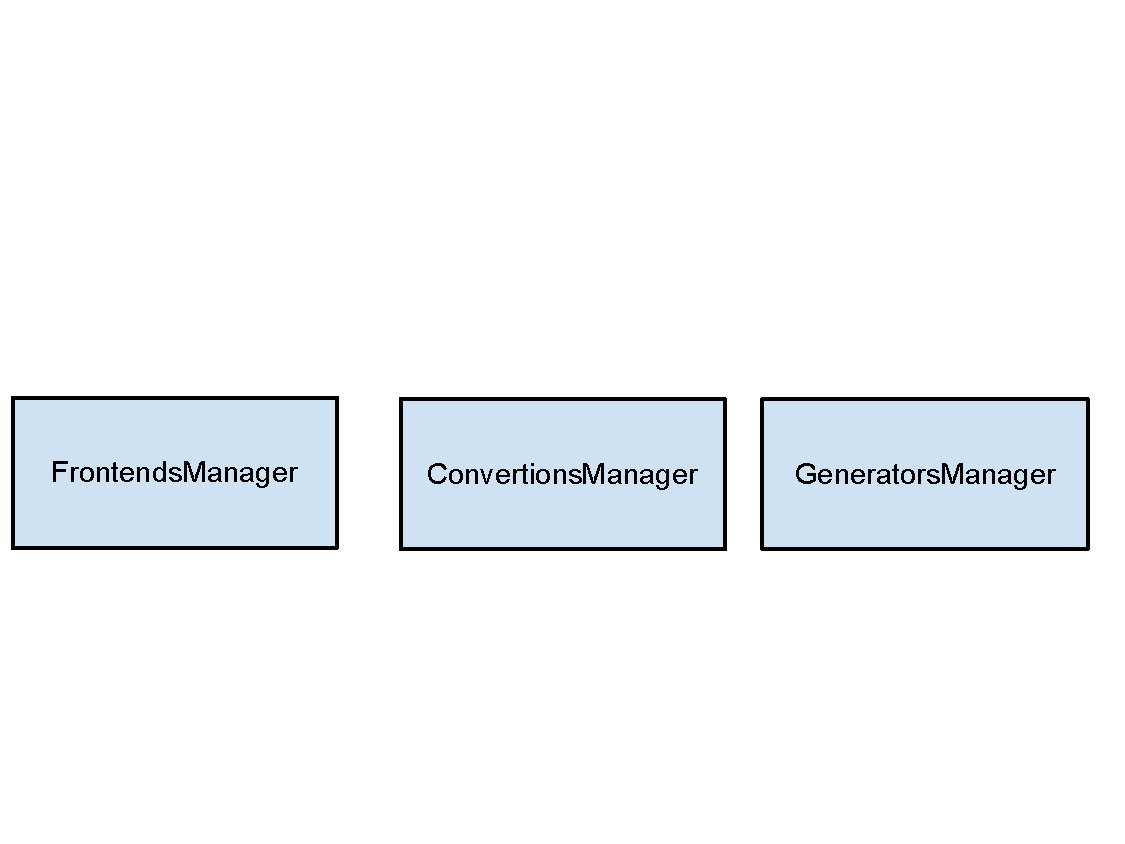
\includegraphics[width= 0.9\textwidth, height=\textheight]{diagrams/YC_old_arch.pdf}}
    \end{center}
\end{frame}    

\begin{frame}
	\transwipe[direction=90]
	\frametitle{Модули YaccConstructor}
	Модули, управляющие загрузкой компонент. Конечый вариант.
	\begin{center}
        {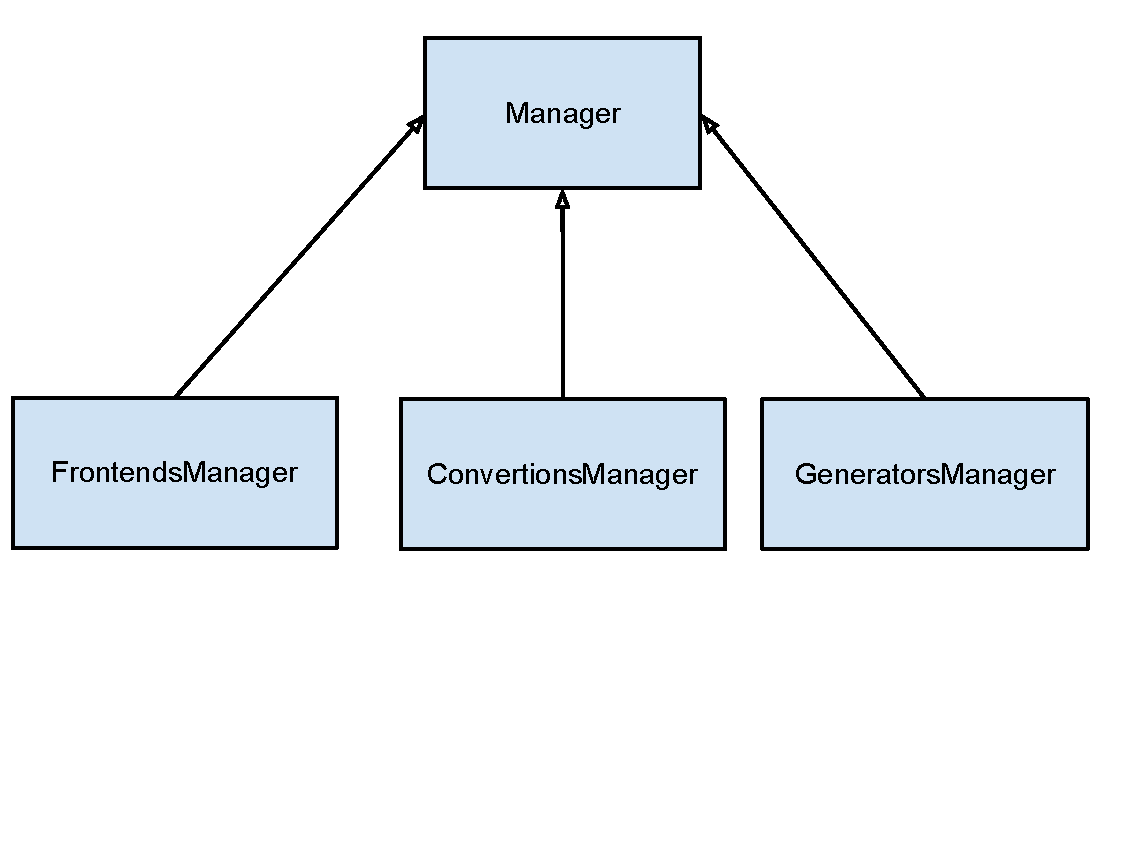
\includegraphics[width= 0.9\textwidth, height=\textheight]{diagrams/YC_new_arch.pdf}}
    \end{center}
\end{frame}    

\begin{frame}
	\transwipe[direction=90]
	\frametitle{Результаты}
	\begin{itemize}
        \item Доработана архитектура модулей загрузки компонент
	    \begin{itemize}
            \item Выявлена общая функциональность модулей
            \item Реализован общий предок с общей функциональностью
        \end{itemize}
        \item Изучены основы языка программирования F\#
        \item Получен опыт работы с системой контроля версий git
        \item Получен опыт разработки unit-тестов и опыт работы с NUnit
    \end{itemize}    
\end{frame}    

\author[Шенбин Илья]{}

\begin{frame}
	\transwipe[direction=90]
	\frametitle{Задача}
	Разработка статических проверок грамматики
	\begin{itemize}
        \item Наличие неописанных нетерминалов
        \item Наличие неиспользуемых нетерминалов
        \item Наличие стартового правила
        \item Наличие ровно одного стартового правила
    \end{itemize}
\end{frame}    

\begin{frame}
	\transwipe[direction=90]
	\frametitle{Процесс работы YaccConstructor}
	\begin{center}
        {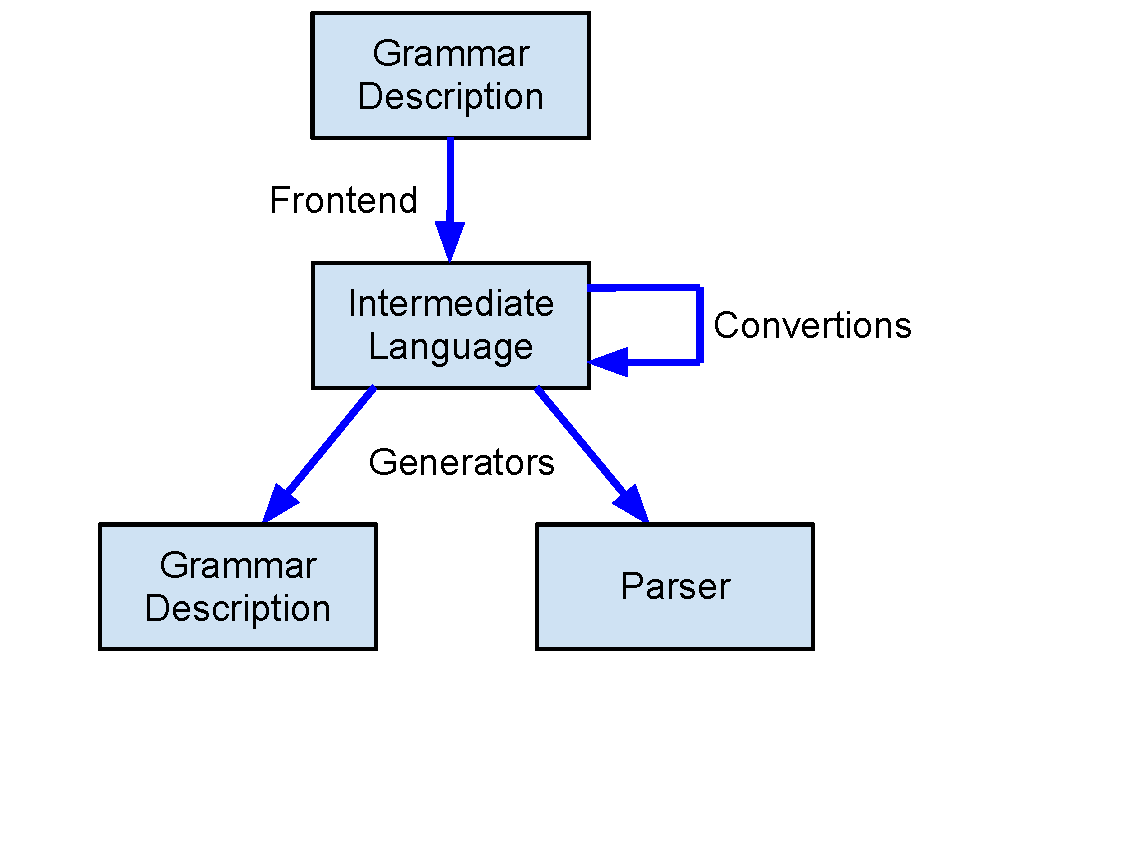
\includegraphics[width= 0.9\textwidth, height=\textheight]{diagrams/YC_workflow_base.pdf}}
    \end{center}
\end{frame}

\begin{frame}
	\transwipe[direction=90]
	\frametitle{Процесс работы YaccConstructor}
	\begin{center}
        {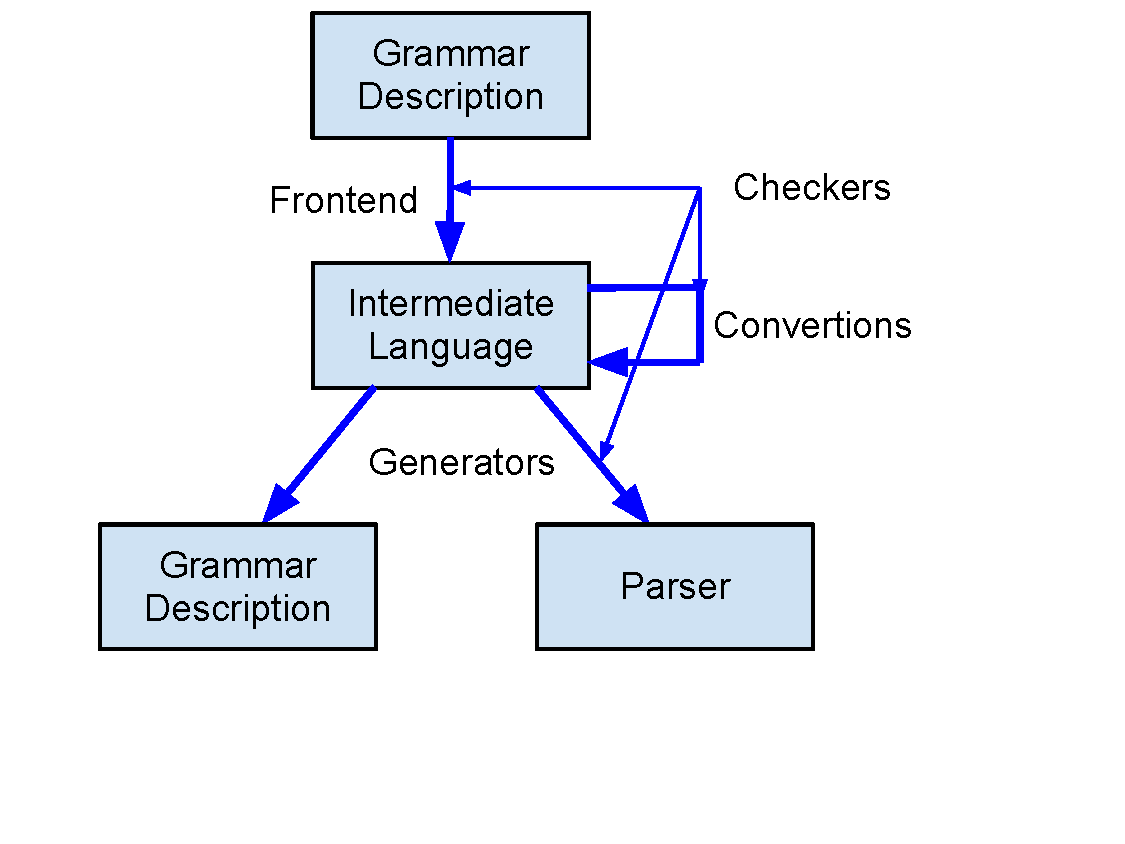
\includegraphics[width= 0.9\textwidth, height=\textheight]{diagrams/YC_workflow_with_checkers.pdf}}
    \end{center}
\end{frame}

\begin{frame}
	\transwipe[direction=90]
	\frametitle{Результаты}
	\begin{itemize}
        \item Разработаны статические провероки грамматики
	    \begin{itemize}
            \item Наличие неописанных нетерминалов
            \item Наличие неиспользуемых нетерминалов
            \item Наличие стартового правила
            \item Наличие ровно одного стартового правила
        \end{itemize}
        \item Изучены основы языка программирования F\#
        \item Получен опыт работы с системой контроля версий git
        \item Получен опыт разработки unit-тестов и опыт работы с NUnit
        \item Получен опыт работы с библиотекой QuickGraph
    \end{itemize}    
\end{frame}
    
\author[Григорьев Семён]{}

\begin{frame}
	\transwipe[direction=90]
	\frametitle{Результаты}
	\begin{itemize}
        \item Используется для разработки парсеров в промышленном проекте.
        \item Основа для исследований кафедры.
    \end{itemize}    
\end{frame}


\begin{frame}
	\transwipe[direction=90]
	\frametitle{Заключение}
	\begin{itemize}
        \item Сайт проекта: \href{http://recursive-ascent.googlecode.com} {http://recursive-ascent.googlecode.com}
	    \item Вопросы, пожелания, предложения: Semen.Grigorev@lanit-tercom.com
    \end{itemize}    
\end{frame}    
    
\end{document}
